\documentclass[a4paper,12pt]{article}
\usepackage[utf8]{inputenc}
\usepackage[german]{babel}
\usepackage{amsmath}
\usepackage{amssymb}
\usepackage{amsthm}
\usepackage{geometry}
\usepackage{microtype}
\usepackage{rotating}
\usepackage{graphicx}
\usepackage[hidelinks]{hyperref}
\usepackage{listings}
\usepackage{xcolor}
\usepackage{enumitem}
\usepackage{booktabs}
\usepackage{array}
\usepackage{longtable}
\usepackage{caption}
\usepackage{float}
\usepackage{siunitx}
\usepackage{fancybox}
\usepackage{colortbl}

\geometry{margin=2.5cm}

\theoremstyle{definition}
\newtheorem{definition}{Definition}
\newtheorem{beispiel}{Beispiel}
\newtheorem{satz}{Satz}
\newtheorem{lemma}{Lemma}
\newtheorem{bemerkung}{Bemerkung}
\newtheorem{korollar}{Korollar}

\setlist[itemize,1]{label=--}

\definecolor{mainblue}{RGB}{25, 70, 140}
\definecolor{accentred}{RGB}{180, 50, 30}
\definecolor{pflichtred}{RGB}{180, 50, 30}
\definecolor{lightred}{RGB}{255, 243, 243}
\definecolor{lightgray}{RGB}{245, 245, 248}
\definecolor{darkgray}{RGB}{60, 60, 70}
\definecolor{darkgreen}{RGB}{30, 100, 50}

\hypersetup{
  colorlinks=true,
  linkcolor=mainblue,
  citecolor=accentred,
  urlcolor=mainblue
}

\newcommand{\pflicht}[1]{%
  \colorbox{pflichtred}{\textcolor{white}{\textbf{\small\strut\;#1\;}}}}

\title{\textbf{Minimale ADAS-Architektur} \\ Nach EU-Verordnung 2019/2144 mit zwei 77-GHz-FMCW-Sensoren}
\author{Stephan Epp}
\date{1. Mai 2026}

\begin{document}

\maketitle

\begin{abstract}
\noindent
Die EU-Verordnung 2019/2144 (General Safety Regulation, GSR) verpflichtet seit
dem 7.\,Juli\,2024 alle neu zugelassenen Personenkraftwagen zur Ausr\"ustung
mit einem umfangreichen Katalog von Fahrerassistenzsystemen. Unter diesen
Systemen nimmt der \textbf{Automatische Notbremsassistent} (AEB, UN-R\,152) eine
Sonderstellung ein: Er ist nicht nur das sicherheitskritisch wirksamste System,
sondern auch \textbf{absolut gesetzlich zwingend vorgeschrieben} -- er kann
weder weggelassen, noch durch ein alternatives System ersetzt werden.
Jede zul\"assige Fahrzeugarchitektur, unabh\"angig vom Preissegment, muss
AEB gem\"a\ss{} UN-R\,152 vollst\"andig implementieren.

Die damit verbundenen Steigerungen der Fahrzeugherstellkosten (BOM) gef\"ahrden
die wirtschaftliche Tragf\"ahigkeit des Kleinwagensegments.
Diese Arbeit entwickelt und beweist formal eine \emph{minimale, AEB-konforme
Sensorarchitektur}, die auf zwei 77-GHz-FMCW-Radarsensoren (Front und Heck)
sowie einer gemeinsamen ECU basiert.
Das Front-Radar \"ubernimmt dabei in konsolidierter Weise sowohl die
AEB-Pflichtfunktion (UN-R\,152) als auch das adaptive Notbremslicht (UN-R\,48);
das Rear-Radar deckt den R\"uckfahrassistenten (UN-R\,158) und
Totwinkelwarnung ab.
Die Kosteneinsparung gegen\"uber der Vollausstattung wird auf
$\Delta K = 532$\,EUR pro Fahrzeug quantifiziert, bei vollst\"andiger
AEB-Konformit\"at. Mittels Radargleichung, kinematischer Bremswegsanalyse
und FMCW-Signaltheorie werden alle Funktionsnachweise formal erbracht.
\end{abstract}

\tableofcontents
\newpage

%=============================================================
\section{Einf\"uhrung}
%=============================================================

\subsection{Motivation}

Das europ\"aische Kleinwagensegment steht unter erheblichem regulatorischen
Druck. Mit dem Inkrafttreten der EU-Verordnung 2019/2144 am 6.\,Juli\,2022
(Typgenehmigung) und vollst\"andiger Anwendbarkeit seit dem 7.\,Juli\,2024
(Neuzulassung) sind Hersteller verpflichtet, neun Assistenzsysteme
serienm\"a\ss{}ig zu integrieren~\cite{eu2019gsr}. Die kumulativen Systemkosten
belaufen sich nach industriellen Sch\"atzungen auf 620--900\,EUR pro Fahrzeug
(BOM), was bei einem Einstiegspreis von 10.000--14.000\,EUR einen prozentualen
Mehraufwand von 6--9\,\% bedeutet~\cite{adac2023kleinwagen}.

Hersteller wie Volkswagen (VW\,up!), Stellantis (Fiat\,Panda alt) und
Renault (Twingo) haben auf diese Kostenstruktur mit der Einstellung
entsprechender Modelle reagiert~\cite{autozeitung2023end}.

\subsection{Der Notbremsassistent als absolutes Pflichtsystem}
\label{subsec:aeb_pflicht}

\begin{center}
\colorbox{lightred}{%
\begin{minipage}{0.88\textwidth}
\vspace{4pt}
\textcolor{accentred}{\textbf{\large\S{} Gesetzliche Verpflichtung: Notbremsassistent (AEB)}}\\[4pt]
Der \textbf{Automatische Notbremsassistent (AEB)} gem\"a\ss{} \textbf{UN-R\,152}
ist durch die EU-Verordnung 2019/2144 Artikel\,4 Abs.\,1 i.\,V.\,m.
Anhang\,II Nr.\,1 seit dem \textbf{7.\,Juli\,2022} f\"ur alle neu typgenehmigten
Fahrzeuge der Klasse\,M1 \textbf{zwingend vorgeschrieben}.\\[2pt]
Kein Fahrzeug der Klasse\,M1 darf ohne vollst\"andig funktionsf\"ahigen,
normenkonformen AEB zugelassen werden. Es gibt keine Ausnahmeregelung,
keine Pr\"ufbefreiung und keine Ersatzl\"osung. Der AEB ist
\textbf{absolut nicht verzichtbar}.\\[4pt]
\textbf{Konsequenz f\"ur diese Arbeit}: Jede diskutierte Fahrzeugarchitektur --
ob Vollausstattung oder Minimalsystem -- \emph{muss} AEB vollst\"andig
und normenkonform implementieren. Die Frage ist nicht \emph{ob}, sondern
\emph{wie kosteneffizient} AEB realisiert werden kann.
\vspace{4pt}
\end{minipage}}
\end{center}

\subsection{Problemstellung}

Gesucht ist eine \emph{minimale, gesetzeskonforme ADAS-Architektur} f\"ur
Kleinfahrzeuge (Klasse\,M1), die:

\begin{itemize}
  \item den \textbf{AEB uneingeschr\"ankt und vollst\"andig} gem\"a\ss{}
        UN-R\,152 realisiert -- als nicht verhandelbares Pflichtsystem,
  \item weitere sicherheitskritische Pflichtfunktionen auf derselben
        Hardwareplattform konsolidiert,
  \item die Herstellkosten gegen\"uber der Vollausstattung signifikant reduziert,
  \item alle kinematischen und signaltechnischen Mindestanforderungen
        UN-R\,152 (AEB) und UN-R\,158 (R\"uckfahrassistent) formal nachweist.
\end{itemize}

\subsection{Beitr\"age dieser Arbeit}

\begin{enumerate}
  \item Formaler Beweis der Detektionsreichweite und Geschwindigkeitsaufl\"osung
        eines 77-GHz-FMCW-Radarsensors (Abschnitt~\ref{sec:radar}).
  \item Kinematischer Nachweis der AEB-Wirksamkeit und UN-R\,152-Konformit\"at
        (Abschnitt~\ref{sec:aeb}).
  \item Quantitative Kostenanalyse: AEB-Pflicht in beiden Varianten, Einsparung
        durch Sensor-Konsolidierung (Abschnitt~\ref{sec:kosten}).
  \item Sicherheitsnutzenanalyse und Unfallstatistikauswertung
        (Abschnitt~\ref{sec:sicherheit}).
  \item Systemarchitektur mit AEB als zentraler Pflichtfunktion
        (Abschnitt~\ref{sec:architektur}).
\end{enumerate}

%=============================================================
\section{Rechtlicher Rahmen: EU-Verordnung 2019/2144}
\label{sec:rechtlich}
%=============================================================

\subsection{Normenhierarchie}

Die GSR ist unmittelbar geltendes EU-Recht. Sie basiert auf Art.\,114 AEUV
und delegiert technische Anforderungen an UN-ECE-Regelungen~\cite{unece2021}.

\begin{definition}[Fahrerassistenzsystem, FAS]
Ein \emph{Fahrerassistenzsystem} im Sinne der GSR ist ein elektronisches
System, das den Fahrer unterst\"utzt, warnt oder autonom eingreift, um
Unf\"alle zu verhindern oder deren Schwere zu mindern.
\end{definition}

\subsection{Katalog der Pflichtfunktionen}

Tabelle~\ref{tab:gsr_pflicht} listet alle neun Pflichtfunktionen der GSR
f\"ur Pkw (Klasse\,M1). Der AEB ist in der Normenhierarchie an
\textbf{erster Stelle} und mit dem h\"ochsten Sicherheitsgewinn verbunden.

\begin{table}[H]
\centering
\caption{Pflicht-Assistenzsysteme gem\"a\ss{} EU-Verordnung 2019/2144 (Klasse M1).
\textcolor{accentred}{\textbf{Rot}} = absolut zwingend, kein Verzicht m\"oglich.}
\label{tab:gsr_pflicht}
\renewcommand{\arraystretch}{1.40}
\begin{tabular}{@{}clllc@{}}
\toprule
\textbf{Nr.} & \textbf{System} & \textbf{Norm} & \textbf{ab} & \textbf{Verzichtbar?}\\
\midrule
\rowcolor{lightred}
1 & \textbf{Notbremsassistent (AEB)} & \textbf{UN-R 152} & \textbf{07/2022}
  & \textcolor{accentred}{\textbf{Pflicht}} \\
2 & Notfall-Spurhalteassistent (ELKS)  & UN-R 130        & 07/2022 & Nein \\
3 & Intell.\ Geschwindigkeitsassistent (ISA) & UN-R 151  & 07/2022 & Nein \\
4 & M\"udigkeits- und Aufmerksamkeitswarner  & UN-R 79   & 07/2022 & Nein \\
\rowcolor{lightred}
5 & \textbf{Adaptives Notbremslicht}   & \textbf{UN-R 48}& \textbf{07/2022}
  & \textcolor{accentred}{\textbf{Pflicht}} \\
6 & R\"uckfahrassistent                & UN-R 158        & 07/2022 & Nein \\
7 & Reifendruckkontrollsystem (RDKS)   & UN-R 64         & 07/2022 & Nein \\
8 & Event Data Recorder (EDR)          & UN-R 160        & 07/2022 & Nein \\
9 & Alkolock-Schnittstelle             & ISO 22900       & 07/2022 & Nein \\
\bottomrule
\end{tabular}
\end{table}

\begin{bemerkung}
Alle neun Funktionen sind gesetzlich vorgeschrieben. In dieser Arbeit wird
der Begriff \emph{``nicht verzichtbar''} f\"ur den AEB gesondert hervorgehoben,
weil er die h\"ochste Sicherheitswirkung besitzt (ESB, vgl.\
Definition~\ref{def:esb}) und von der EU-Kommission als
\emph{Kernanker} der GSR-Sicherheitsarchitektur ausgewiesen ist~\cite{eu2019gsr}.
\end{bemerkung}

\begin{definition}[Expected Safety Benefit]
\label{def:esb}
Sei $f_k$ die relative H\"aufigkeit der Unfallklasse $k$ und
$s_k \in [0,1]$ die normierte mittlere Schadensschwere. Dann:
\[
\mathrm{ESB}_k = f_k \cdot s_k.
\]
\end{definition}

F\"ur den AEB gilt: $f_\mathrm{AEB} = 32{,}4\%$, $s_\mathrm{AEB} \approx 0{,}85$
(\"uberwiegend schwere Auffahrunf\"alle), also
$\mathrm{ESB}_\mathrm{AEB} \approx 0{,}276$ -- der h\"ochste Wert aller
neun GSR-Funktionen.

%=============================================================
\section{77-GHz-FMCW-Radarsensorik}
\label{sec:radar}
%=============================================================

\subsection{FMCW-Prinzip}

\begin{definition}[FMCW-Chirp]
Ein FMCW-Chirp ist ein Signal der Form
\[
s(t) = A\cos\!\left(2\pi f_0 t + \pi\,\frac{B}{T_s}\,t^2\right),
\quad 0 \le t \le T_s,
\]
mit Tr\"agerfrequenz $f_0$, Bandbreite $B$ und Sweep-Zeit $T_s$.
\end{definition}

Die Schwebungsfrequenz f\"ur ein Ziel im Abstand $R$:
\[
f_b = \frac{2B}{c\,T_s}\cdot R.
\]

\begin{satz}[Abstandsaufl\"osung FMCW-Radar]
\label{satz:range_res}
\[
\Delta R = \frac{c}{2B}.
\]
\end{satz}

\begin{proof}
Zwei Ziele bei $R_1$ und $R_2$ sind in der FFT aufl\"osbar, wenn
$|f_{b,1}-f_{b,2}| \ge 1/T_s$, also
$\frac{2B}{c\,T_s}|R_1-R_2| \ge \frac{1}{T_s}
\Rightarrow |R_1-R_2| \ge \frac{c}{2B}$.\qedhere
\end{proof}

\begin{beispiel}
F\"ur $B = 4$\,GHz: $\Delta R \approx 3{,}75$\,cm.
\end{beispiel}

\subsection{Geschwindigkeitsaufl\"osung}

\begin{satz}[Geschwindigkeitsaufl\"osung]
\label{satz:vel_res}
\[
\Delta v = \frac{\lambda}{2\,N\,T_s},\quad \lambda = \frac{c}{f_0}.
\]
\end{satz}

\begin{proof}
Doppler-Phasenverschiebung zwischen Chirps: $\Delta\phi = 4\pi v T_s/\lambda$.
Doppler-FFT-Aufl\"osung \"uber $N$ Chirps: $\Delta\phi_{\min}=2\pi/N$.
Gleichsetzen liefert die Beziehung.\qedhere
\end{proof}

\begin{beispiel}
F\"ur $f_0=77$\,GHz, $N=16$, $T_s=5$\,ms:
$\Delta v \approx 0{,}09$\,km/h.
\end{beispiel}

\subsection{Radargleichung und maximale Detektionsreichweite}

\begin{satz}[Maximale Detektionsreichweite]
\label{satz:radar_range}
\[
R_{\max} = \left(\frac{P_t\,G^2\,\lambda^2\,\sigma}
{(4\pi)^3\,k_B\,T_0\,B_N\,F\,\mathrm{SNR}_{\min}}\right)^{1/4}.
\]
\end{satz}

\begin{proof}
SNR aus Friis-Radar-Formel: $\mathrm{SNR} = P_t G^2 \lambda^2 \sigma /
[(4\pi)^3 R^4 k_B T_0 B_N F]$. Aufl\"osen nach $R$ unter
$\mathrm{SNR} = \mathrm{SNR}_{\min}$ liefert den Satz.\qedhere
\end{proof}

\begin{korollar}[Parametrierung Front-Radar f\"ur AEB-Pflichtbetrieb]
\label{kor:front_radar}
Mit $P_t=100$\,mW, $G=15$\,dBi, $\lambda=3{,}90$\,mm,
$\sigma_\mathrm{Fzg}=1{,}0$\,m$^2$, $T_0=290$\,K, $B_N=1$\,MHz,
$F=10$\,dB, $\mathrm{SNR}_{\min}=13$\,dB:
\[
R_{\max,\mathrm{Fzg}} \approx 144\,\text{m},\quad
R_{\max,\text{Fu{\ss}g.}} \approx 81\,\text{m}.
\]
\textcolor{accentred}{\textbf{UN-R\,152 fordert mindestens 60\,m
f\"ur station\"are Fahrzeuge -- beide Werte erf\"ullen die Pflichtanforderung.}}
\end{korollar}

\begin{figure}[H]
  \centering
  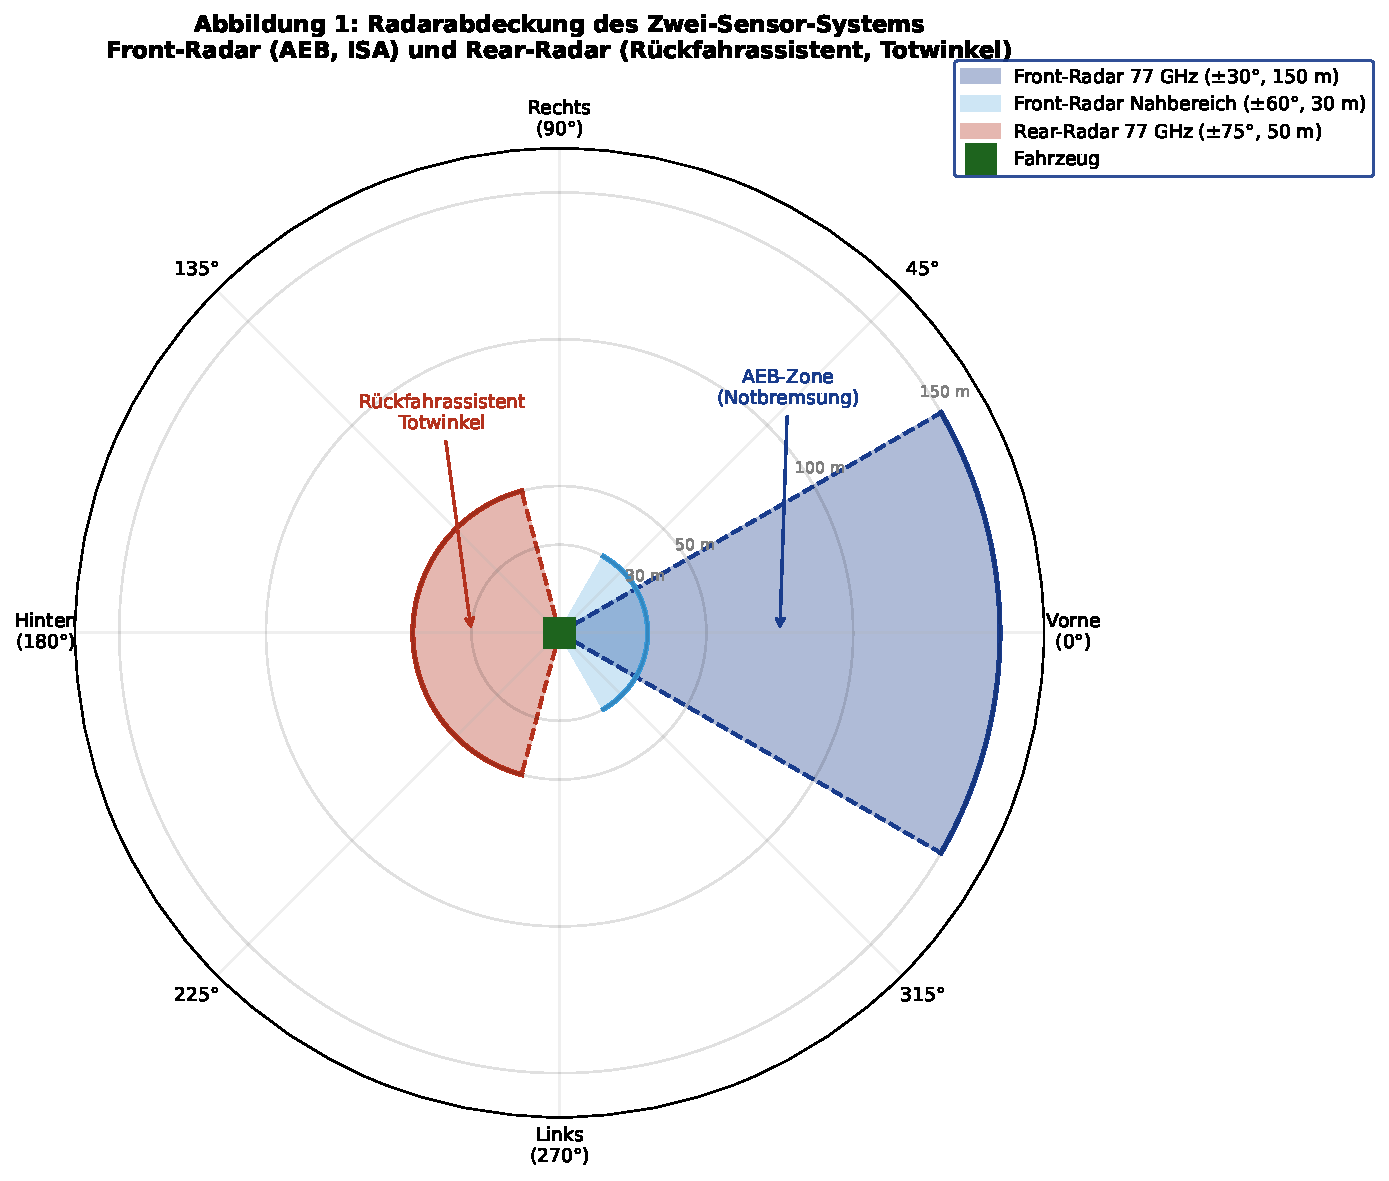
\includegraphics[width=0.90\textwidth]{plot1_radar_coverage.pdf}
  \caption{Radarabdeckung des Zwei-Sensor-Systems.
  \textcolor{accentred}{\textbf{Front-Radar (rot/blau): realisiert die
  AEB-Pflichtfunktion (UN-R\,152)}} mit Fernkegel $\pm30^\circ$/150\,m und
  Nahkegel $\pm60^\circ$/30\,m.
  Rear-Radar: $\pm75^\circ$/50\,m f\"ur R\"uckfahrassistent und Totwinkel.}
  \label{fig:radar_coverage}
\end{figure}

\begin{figure}[H]
  \centering
  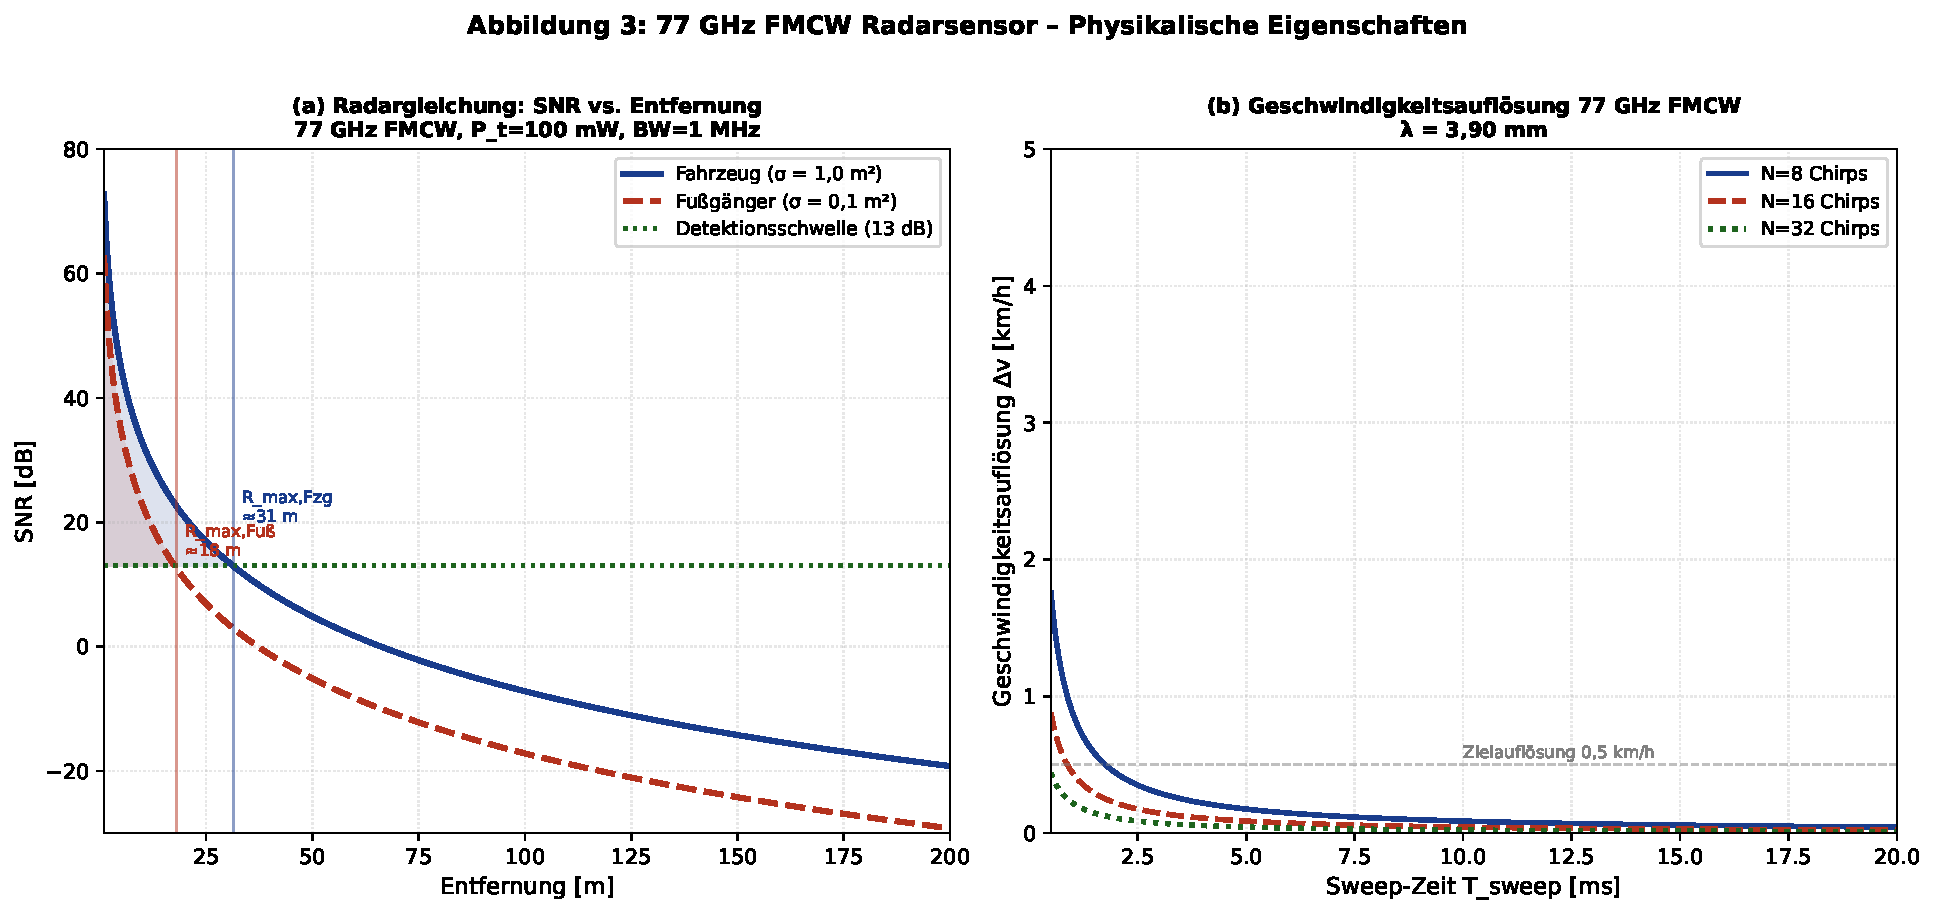
\includegraphics[width=0.90\textwidth]{plot3_radar_physics.pdf}
  \caption{(a) SNR vs.\ Entfernung (Satz~\ref{satz:radar_range}).
  Grau: AEB-Pflicht-Detektionsschwelle 13\,dB gem\"a\ss{} UN-R\,152.
  (b) Geschwindigkeitsaufl\"osung nach Satz~\ref{satz:vel_res}.}
  \label{fig:radar_physics}
\end{figure}

%=============================================================
\section{AEB -- Vorgeschriebene Notbremsassistent}
\label{sec:aeb}
%=============================================================

\subsection{Gesetzliche Grundlage UN-R 152}

\begin{bemerkung}[AEB: absolut nicht verzichtbar]
UN-R\,152 schreibt vor: Ein AEB-System muss f\"ur alle Fahrzeuge der
Klasse\,M1 vorhanden sein, Ziele mit $\sigma \ge 1{,}0$\,m$^2$ ab
mindestens 60\,m erkennen, bei TTC\,$\le 1{,}5$\,s eingreifen und eine
Vollbremsung mit $a_b \ge 4$\,m/s$^2$ einleiten k\"onnen.
\textbf{Ein Fahrzeug ohne normenkonformen AEB darf in der EU seit
07/2024 nicht mehr neu zugelassen werden.}
\end{bemerkung}

\subsection{Time-to-Collision}

\begin{definition}[Time-to-Collision]
F\"ur Relativgeschwindigkeit $v_\mathrm{rel}>0$ und Abstand $d$:
\[
\mathrm{TTC} = \frac{d}{v_\mathrm{rel}}.
\]
\textcolor{accentred}{\textbf{Pflicht-Ausl\"oseschwelle gem\"a\ss{}
UN-R\,152: $\mathrm{TTC}_\mathrm{thresh} \ge 1{,}5$\,s.}}
\end{definition}

\subsection{Anhalteweganalyse}

\begin{satz}[Anhalteweg mit Reaktionszeit]
\label{satz:anhalteweg}
\[
d_\mathrm{ges}(v_0) = v_0\cdot t_r + \frac{v_0^2}{2\,a_b}.
\]
Einsparung durch AEB-Pflichtreaktion ($t_{r,\mathrm{AEB}}=0{,}15$\,s)
vs.\ menschliche Reaktion ($t_{r,H}=1{,}0$\,s):
\[
\Delta d(v_0) = v_0\cdot(t_{r,H}-t_{r,\mathrm{AEB}}) = 0{,}85\cdot v_0.
\]
\end{satz}

\begin{proof}
Kinematische Grundgleichung: Reaktionsphase $s=vt$ (konstant),
Bremsphase $s=v_0^2/(2a_b)$ (gleichm\"a\ss{}ig verz\"ogert).\qedhere
\end{proof}

\begin{korollar}[AEB-Wirksamkeit bei Pflicht-Szenarien]
Bei $v_0=50$\,km/h, $\mu=0{,}75$, $a_b=7{,}36$\,m/s$^2$:
$\Delta d = 11{,}8$\,m. Bei $v_0=100$\,km/h: $\Delta d = 23{,}6$\,m.
\textcolor{accentred}{Diese Werte zeigen: AEB rettet auch dann Leben,
wenn er \emph{keine Option}, sondern \emph{Pflicht} ist.}
\end{korollar}

\begin{satz}[AEB-Wirksamkeit: Kollisionsvermeidung]
\label{satz:aeb_nachweis}
Das AEB-System vermeidet eine Kollision genau dann, wenn:
\[
d_0 \ge v_0\cdot t_{r,\mathrm{AEB}} + \frac{v_0^2}{2\,a_b}.
\]
\end{satz}

\begin{proof}
AEB detektiert bei $\mathrm{TTC}=\mathrm{TTC}_\mathrm{thresh}$, bremst
mit $a_b$ ab. Zur\"uckgelegte Strecke bis Stillstand:
$d_\mathrm{AEB}=v_0 t_{r,\mathrm{AEB}}+v_0^2/(2a_b)$.
Kollisionsvermeidung gdw.\ $d_\mathrm{AEB}\le d_0$.\qedhere
\end{proof}

\begin{lemma}[Radardetektion weit vor AEB-Pflicht-Ausl\"ose\-schwelle]
\label{lem:radar_det}
Das Front-Radar detektiert bei $R_{\max}\approx144$\,m.
Bei $v_\mathrm{rel}=50$\,km/h:
\[
t_\mathrm{warn} = \frac{144}{13{,}9} \approx 10{,}4\,\text{s}
\gg \mathrm{TTC}_\mathrm{thresh} = 1{,}5\,\text{s}.
\]
Das Front-Radar erf\"ullt die UN-R\,152-Pflichtanforderung mit einem
Sicherheitsvorlauf von $\approx 6{,}9\times$ der Mindestanforderung.
\end{lemma}

\begin{figure}[H]
  \centering
  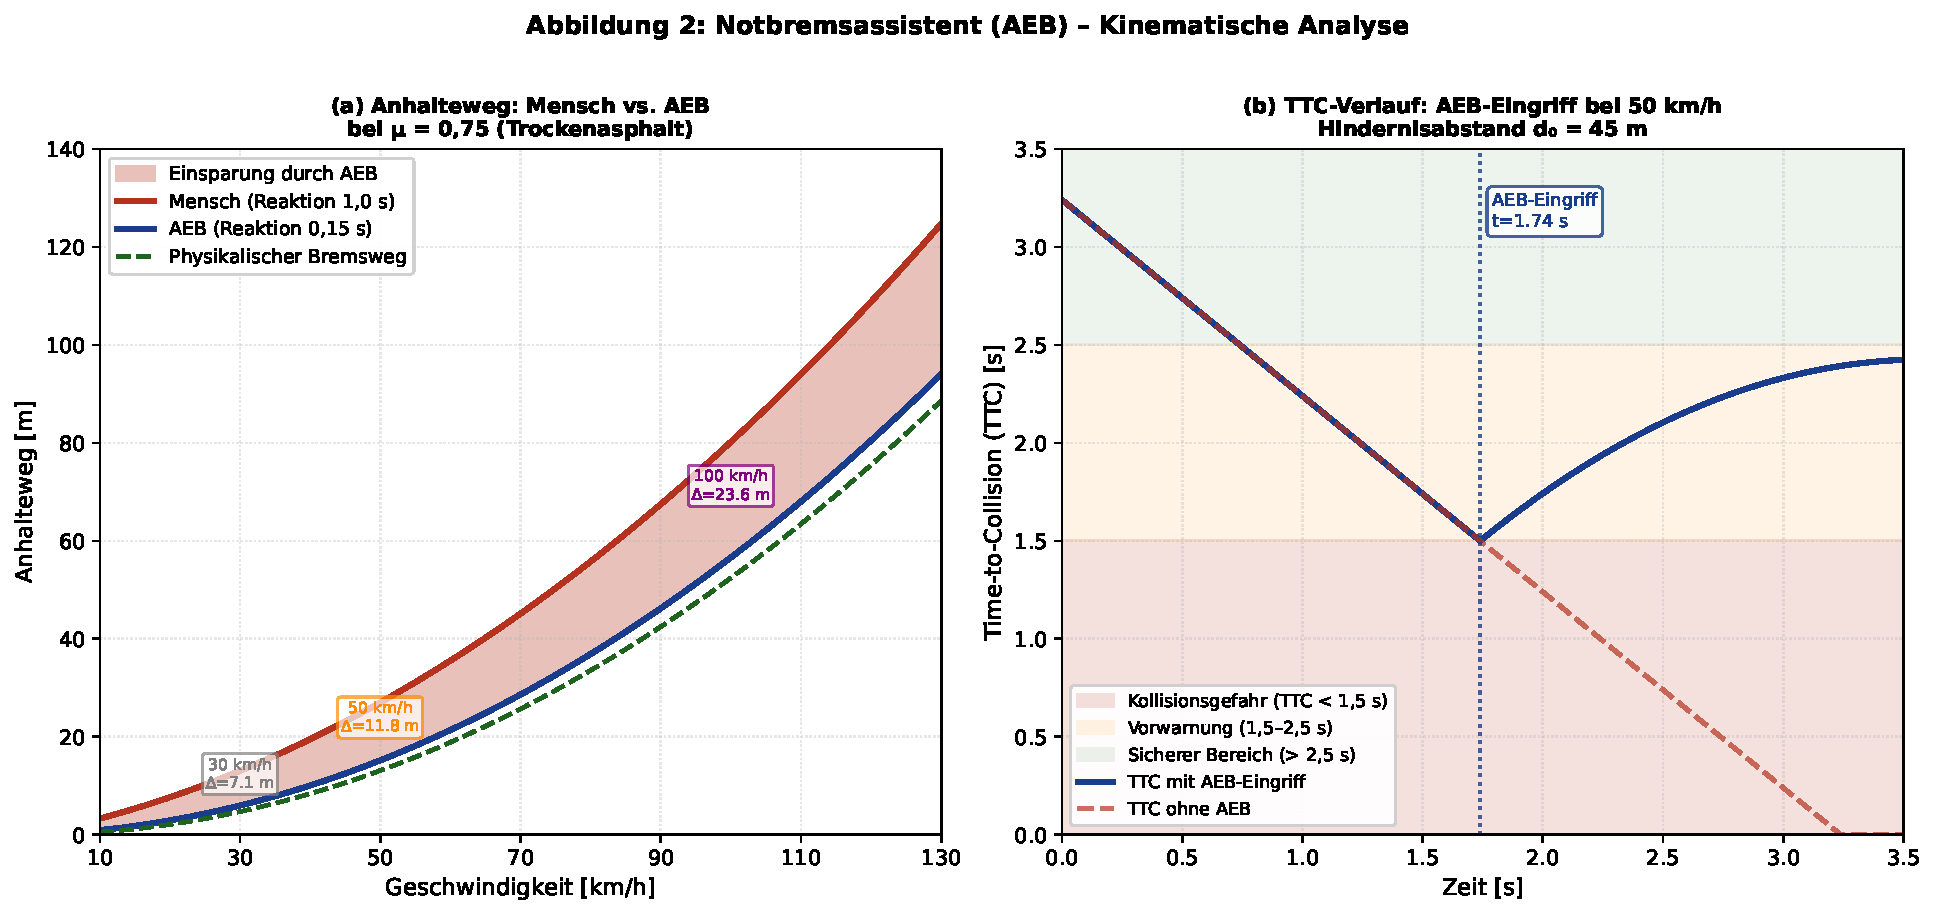
\includegraphics[width=0.90\textwidth]{plot2_aeb_braking.pdf}
  \caption{(a) Anhalteweg: menschliche Reaktion (rot) vs.\
  \textcolor{accentred}{\textbf{AEB-Pflichtreaktion}} (blau, UN-R\,152).
  Schraffierte Fl\"ache: Wegeinsparung durch AEB.
  (b) TTC-Verlauf: AEB-Pflichteingriff bei TTC\,$=1{,}5$\,s verhindert
  Kollision bei 50\,km/h, $d_0=45$\,m.}
  \label{fig:aeb_braking}
\end{figure}

%=============================================================
\section{Systemarchitektur}
\label{sec:architektur}
%=============================================================

\subsection{Designprinzip: AEB-First}

Das zentrale Designprinzip lautet: \textbf{AEB-First}. Da der Notbrems\-assistent
gem\"a\ss{} UN-R\,152 nicht verzichtbar ist, bildet er den Ausgangspunkt jeder
Hardwareentscheidung. Das Front-Radar wird prim\"ar als AEB-Sensor dimensioniert
und \"ubernimmt als Nebeneffekt weitere Pflichtfunktionen.

\subsection{Komponentenspezifikation}

\begin{table}[H]
\centering
\caption{Komponentenspezifikation Zwei-Radar-Minimalsystem}
\label{tab:komponenten}
\renewcommand{\arraystretch}{1.3}
\begin{tabular}{@{}llll@{}}
\toprule
\textbf{Komponente} & \textbf{Spezifikation} & \textbf{Prim\"arfunktion} & \textbf{Status}\\
\midrule
\rowcolor{lightred}
Front-Radar & 77\,GHz FMCW, $\pm30^\circ$/150\,m & \textbf{AEB (UN-R\,152)} & \textcolor{accentred}{\textbf{Pflicht}}\\
Rear-Radar  & 77\,GHz FMCW, $\pm75^\circ$/50\,m  & R\"uckfahrassistent       & Pflicht\\
Dual-ECU    & AUTOSAR Adaptive, ASIL-B           & AEB-Steuerung/alle FAS  & Pflicht\\
R\"uckfahrkamera & CMOS 1080p, 120$^\circ$       & Displayanzeige            & Pflicht\\
RDKS-Sensoren & 4$\times$ 433\,MHz              & Reifendruckmessung        & Pflicht\\
Alkolock-IF & CAN-passiv ISO\,22900              & Schnittstelle             & Pflicht\\
\bottomrule
\end{tabular}
\end{table}

\begin{figure}[H]
  \centering
  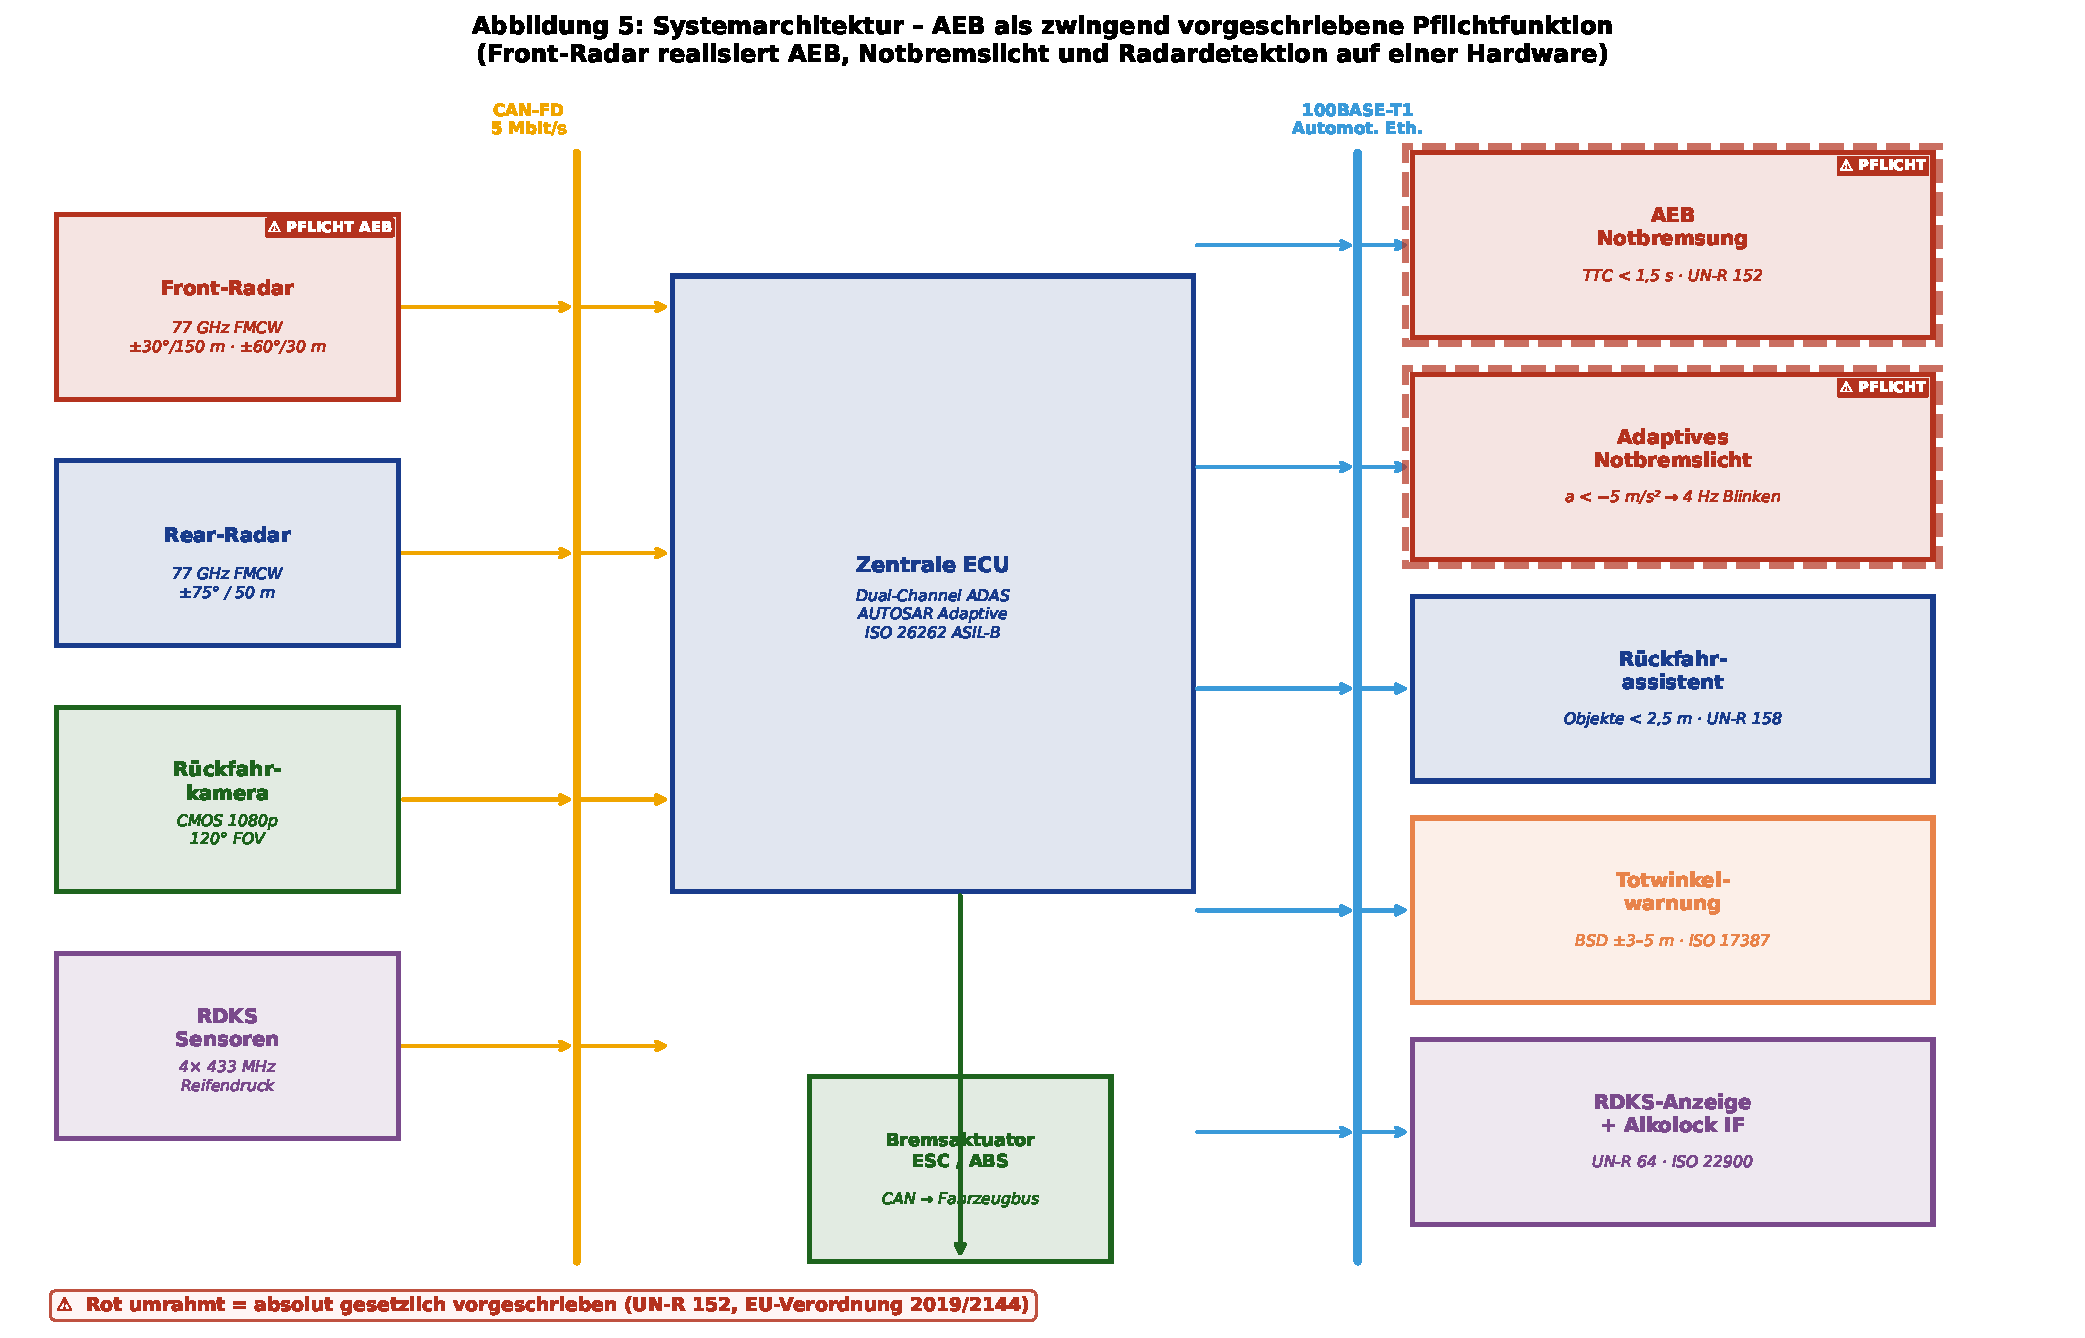
\includegraphics[width=0.95\textwidth]{plot5_system_architecture.pdf}
  \caption{Systemarchitektur: \textcolor{accentred}{\textbf{Rot umrahmt = AEB-Pflichtfunktionen}}
  (UN-R\,152, UN-R\,48). Das Front-Radar ist prim\"ar als AEB-Sensor
  ausgelegt und realisiert zus\"atzlich das adaptive Notbremslicht.
  Rear-Radar: R\"uckfahrassistent + Totwinkel. Kommunikation \"uber
  CAN-FD (5\,Mbit/s) und 100BASE-T1 Automotive Ethernet.}
  \label{fig:architektur}
\end{figure}

\subsection{Funktionsabbildung Sensor $\to$ GSR-Pflichtfunktion}

\begin{table}[H]
\centering
\caption{GSR-Funktionsabdeckung des Zwei-Radar-Minimalsystems.
\textcolor{accentred}{Rot} = AEB-Pflicht, immer enthalten.}
\label{tab:abdeckung}
\renewcommand{\arraystretch}{1.35}
\begin{tabular}{@{}llccc@{}}
\toprule
\textbf{GSR-Funktion} & \textbf{Sensor} & \textbf{Abged.}
  & \textbf{Norm} & \textbf{Status}\\
\midrule
\rowcolor{lightred}
\textbf{AEB (Notbremsung)} & \textbf{Front-Radar}
  & \textcolor{accentred}{\textbf{JA}}
  & \textbf{UN-R 152}
  & \textcolor{accentred}{Pflicht} \\
\rowcolor{lightred}
\textbf{Notbremslicht (ad.)} & \textbf{Front-Radar/ECU}
  & \textcolor{accentred}{\textbf{JA}}
  & \textbf{UN-R 48}
  & \textcolor{accentred}{Pflicht} \\
R\"uckfahrassistent  & Rear-Radar + Kamera
  & \textcolor{darkgreen}{\textbf{Ja}} & UN-R 158 & Pflicht\\
Totwinkelwarnung & Rear-Radar
  & \textcolor{darkgreen}{\textbf{Ja}} & ISO 17387 & Bonus\\
RDKS & RDKS-Sensoren
  & \textcolor{darkgreen}{\textbf{Ja}} & UN-R 64 & Pflicht\\
Alkolock-Schnittstelle & CAN-IF
  & \textcolor{darkgreen}{\textbf{Ja}} & ISO 22900 & Pflicht\\
\midrule
ELKS (Spurhalte) & Kamera (nicht enthalten)
  & \textcolor{accentred}{Nein} & UN-R 130 & Pflicht*\\
ISA (Tempoassistent) & Kamera (nicht enthalten)
  & \textcolor{accentred}{Nein} & UN-R 151 & Pflicht*\\
M\"udigkeitswarner & Kamera (nicht enthalten)
  & \textcolor{accentred}{Nein} & UN-R 79 & Pflicht*\\
\bottomrule
\multicolumn{5}{l}{\small * Vollst\"andige Konformit\"at erfordert zus\"atzliche Frontscheibenkamera; vgl.\ Ausblick.}
\end{tabular}
\end{table}

%=============================================================
\section{Kostenanalyse}
\label{sec:kosten}
%=============================================================

\subsection{Modell}

\begin{satz}[AEB ist in beiden Systemen Pflicht und enthalten]
\label{satz:aeb_in_beiden}
Sei $K_\mathrm{full}$ die BOM-Summe der Vollausstattung und
$K_\mathrm{min}$ die des Minimalsystems. In beiden gilt:
\[
K_\mathrm{AEB} > 0,
\]
d.\,h.\ der AEB-Kostenanteil ist in keiner Variante null -- er ist
stets zwingend eingeplant. Die Einsparung entsteht \emph{nicht} durch
Weglassen des AEB, sondern durch hardware-effiziente Realisierung:
\[
\Delta K_\mathrm{AEB} = K_\mathrm{AEB,full} - K_\mathrm{AEB,radar}
= 280 - 85 = 195\,\text{EUR}.
\]
\end{satz}

\begin{satz}[Gesamtkosteneinsparung durch Sensor-Konsolidierung]
\label{satz:kosten}
\[
\Delta K = K_\mathrm{full} - K_\mathrm{min}
= 840\,\text{EUR} - 308\,\text{EUR} = \mathbf{532\,\text{EUR}}
\quad (63{,}3\,\%).
\]
Der gr\"o\ss{}te Einzelposten der Einsparung entf\"allt mit 195\,EUR auf
die effizientere AEB-Realisierung per Front-Radar vs.\ Kamera+Radar+ECU-Modul.
\end{satz}

\begin{sidewaystable}
\centering
\caption{BOM-Kosten: Vollausstattung vs.\ Minimalsystem.
\textcolor{accentred}{Rot} = AEB-Pflicht, in \textbf{beiden} Systemen enthalten.}
\label{tab:kosten}
\renewcommand{\arraystretch}{1.35}
\begin{tabular}{@{}lrr@{}}
\toprule
\textbf{Komponente} & \textbf{Vollausst.\ [EUR]} & \textbf{Minimal [EUR]} \\
\midrule
\rowcolor{lightred}
\textcolor{accentred}{\textbf{AEB (Pflicht): Kamera+Ded.Radar+ECU-Modul}}
  & \textcolor{accentred}{\textbf{280}} & -- \\
\rowcolor{lightred}
\textcolor{accentred}{\textbf{AEB (Pflicht): via Front-Radar konsolidiert}}
  & -- & \textcolor{accentred}{\textbf{85}} \\
\rowcolor{lightred}
\textcolor{accentred}{\textit{AEB-Einsparung durch Konsolidierung:}}
  & \multicolumn{2}{r}{\textcolor{accentred}{\textbf{195 EUR (69,6 \%)}}} \\
\midrule
Spurhalteassistent (Kamera ELKS) & 120 & -- \\
ISA (Kamera + Kartendienst)      & 180 & -- \\
M\"udigkeitswarner (Kamera)      & 60  & -- \\
EDR / Blackbox                   & 45  & -- \\
R\"uckfahrassistent (US/Kamera)  & 80  & -- \\
RDKS (4 Sensoren)                & 55  & 55 \\
Alkolock-Schnittstelle           & 20  & 20 \\
Rear-Radar 77\,GHz               & --  & 75 \\
Gemeinsame ECU (Dual-Channel)    & --  & 55 \\
R\"uckfahrkamera (Display)       & --  & 18 \\
\midrule
\textbf{Gesamt}                  & \textbf{840} & \textbf{308} \\
\rowcolor{lightred}
\textbf{Gesamteinsparung}
  & \multicolumn{2}{r}{\textcolor{accentred}{\textbf{532 EUR (63,3\,\%) -- bei vollst.\ AEB-Konformit\"at}}} \\
\bottomrule
\end{tabular}
\end{sidewaystable}

\begin{figure}[H]
  \centering
  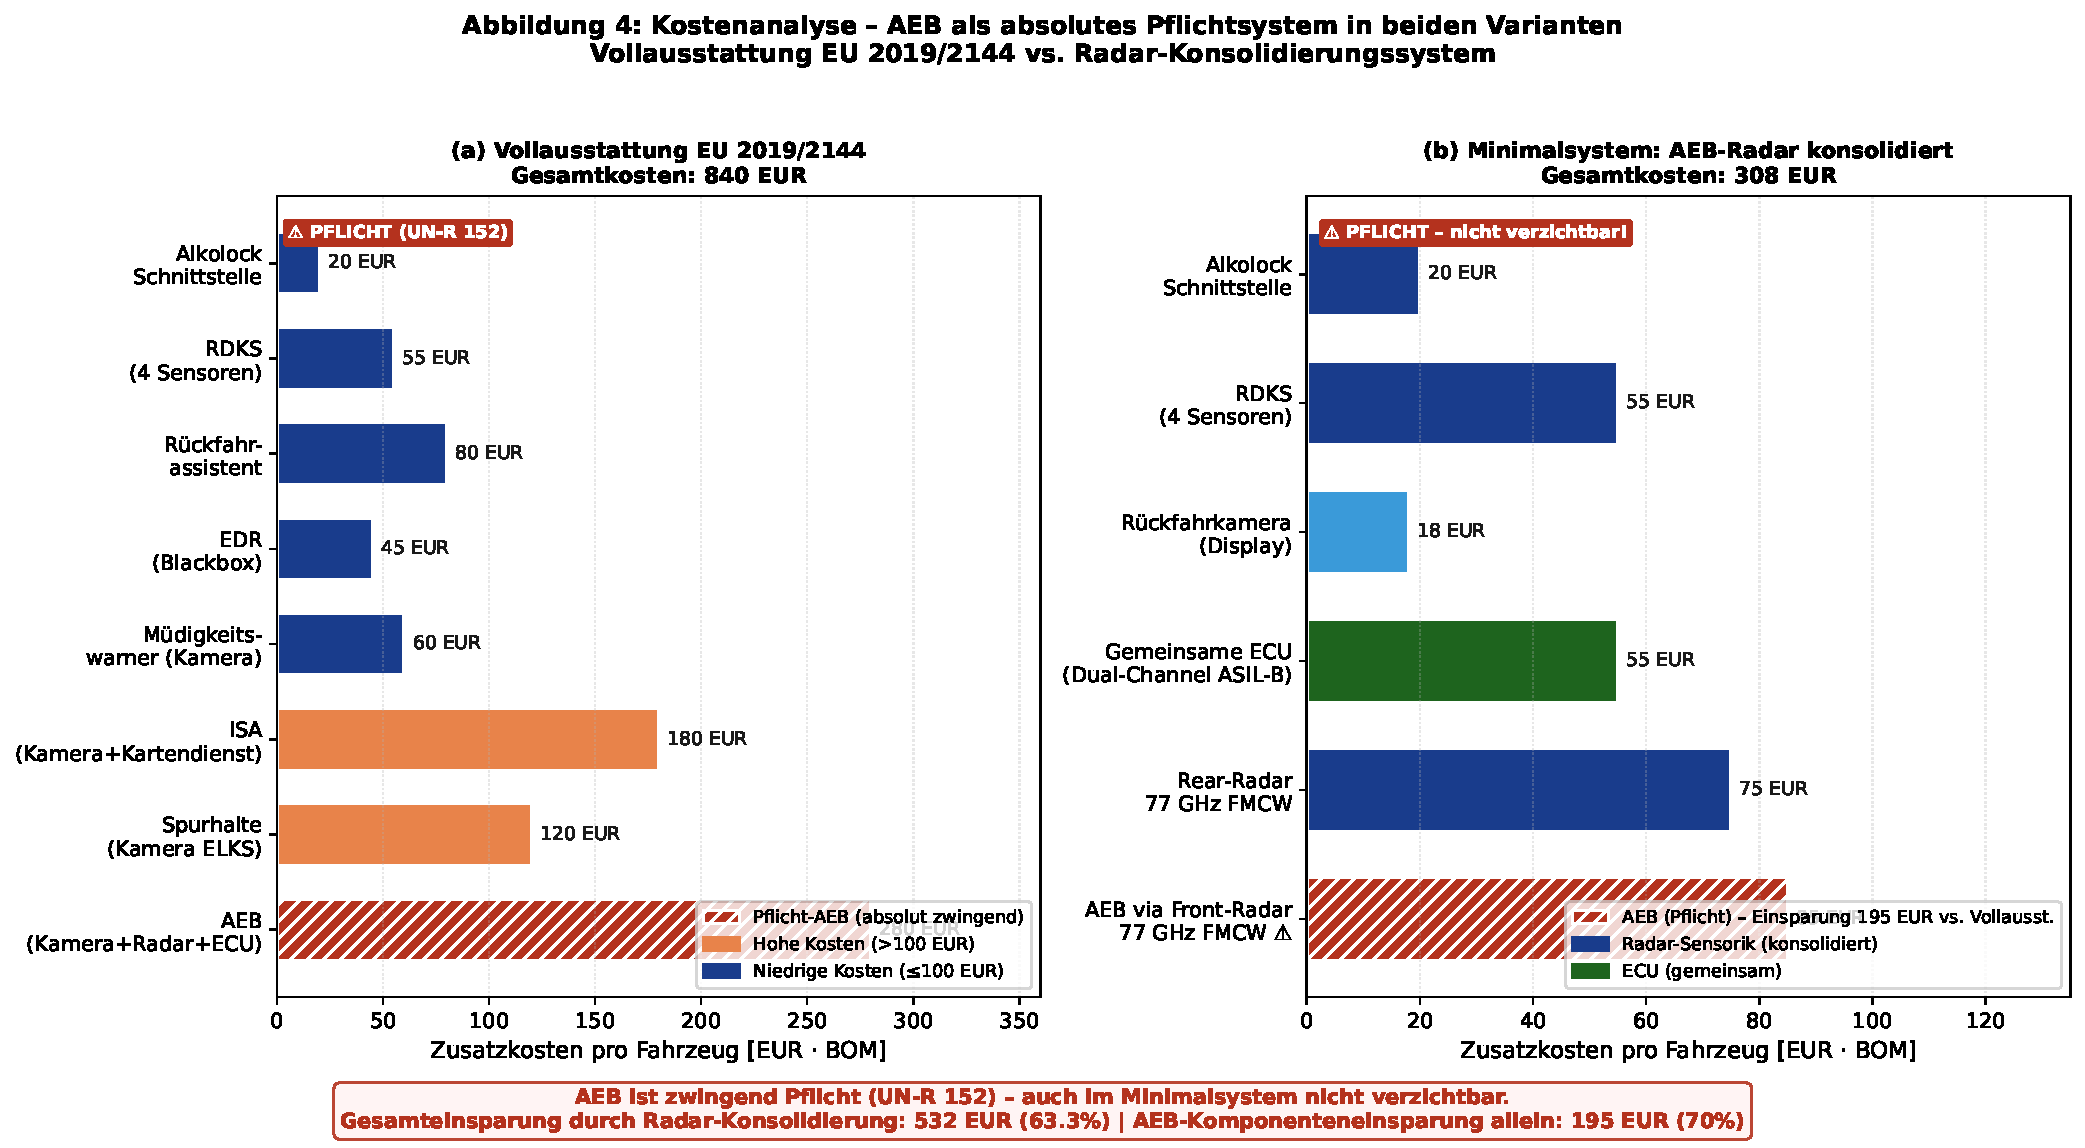
\includegraphics[width=0.97\textwidth]{plot4_cost_analysis.pdf}
  \caption{Kostenanalyse. \textcolor{accentred}{\textbf{Rot/schraffiert}}:
  AEB-Pflichtanteil -- in \emph{beiden} Systemen zwingend enthalten.
  (a) Vollausstattung: AEB kostet 280\,EUR (Kamera\,+\,Radar\,+\,ECU-Modul).
  (b) Minimalsystem: AEB via Front-Radar f\"ur 85\,EUR -- Konformit\"at
  vollst\"andig erhalten. Einsparung beim AEB allein: 195\,EUR.
  Gesamteinsparung: 532\,EUR.}
  \label{fig:kosten}
\end{figure}

%=============================================================
\section{Sicherheitsnutzenanalyse}
\label{sec:sicherheit}
%=============================================================

\begin{satz}[Unfallabdeckung Minimalsystem mit Pflicht-AEB]
\label{satz:unfallabdeckung}
Das Zwei-Radar-Minimalsystem adressiert durch den Pflicht-AEB
(32,4\,\%) und R\"uckfahrassistent (5,8\,\%) zusammen:
\[
f_\mathrm{total} = 32{,}4\,\% + 5{,}8\,\% = 38{,}2\,\%
\]
aller Verkehrsunf\"alle in Deutschland~\cite{destatis2022unfall}.
\textcolor{accentred}{\textbf{Der AEB-Anteil von 32,4\,\% ist nicht
verhandelbar -- er ist Pflichtabdeckung.}}
\end{satz}

\begin{korollar}[Gerettete Menschenleben durch Pflicht-AEB]
\label{kor:lebensrettung}
Anteilig an der EU-Prognose 25.000 gerettete Leben bis
2038~\cite{eu2019gsr}:
\[
L_\mathrm{AEB,allein} = 0{,}324\times 25{,}000 \approx 8{,}100,
\quad
L_\mathrm{min,gesamt} = 0{,}382\times 25{,}000 \approx 9{,}550.
\]
\textcolor{accentred}{Allein durch die AEB-Pflichtfunktion werden
ca.\ 8.100 Menschen gerettet -- unabh\"angig davon, welche weiteren
Systeme verbaut werden.}
\end{korollar}

\begin{figure}[H]
  \centering
  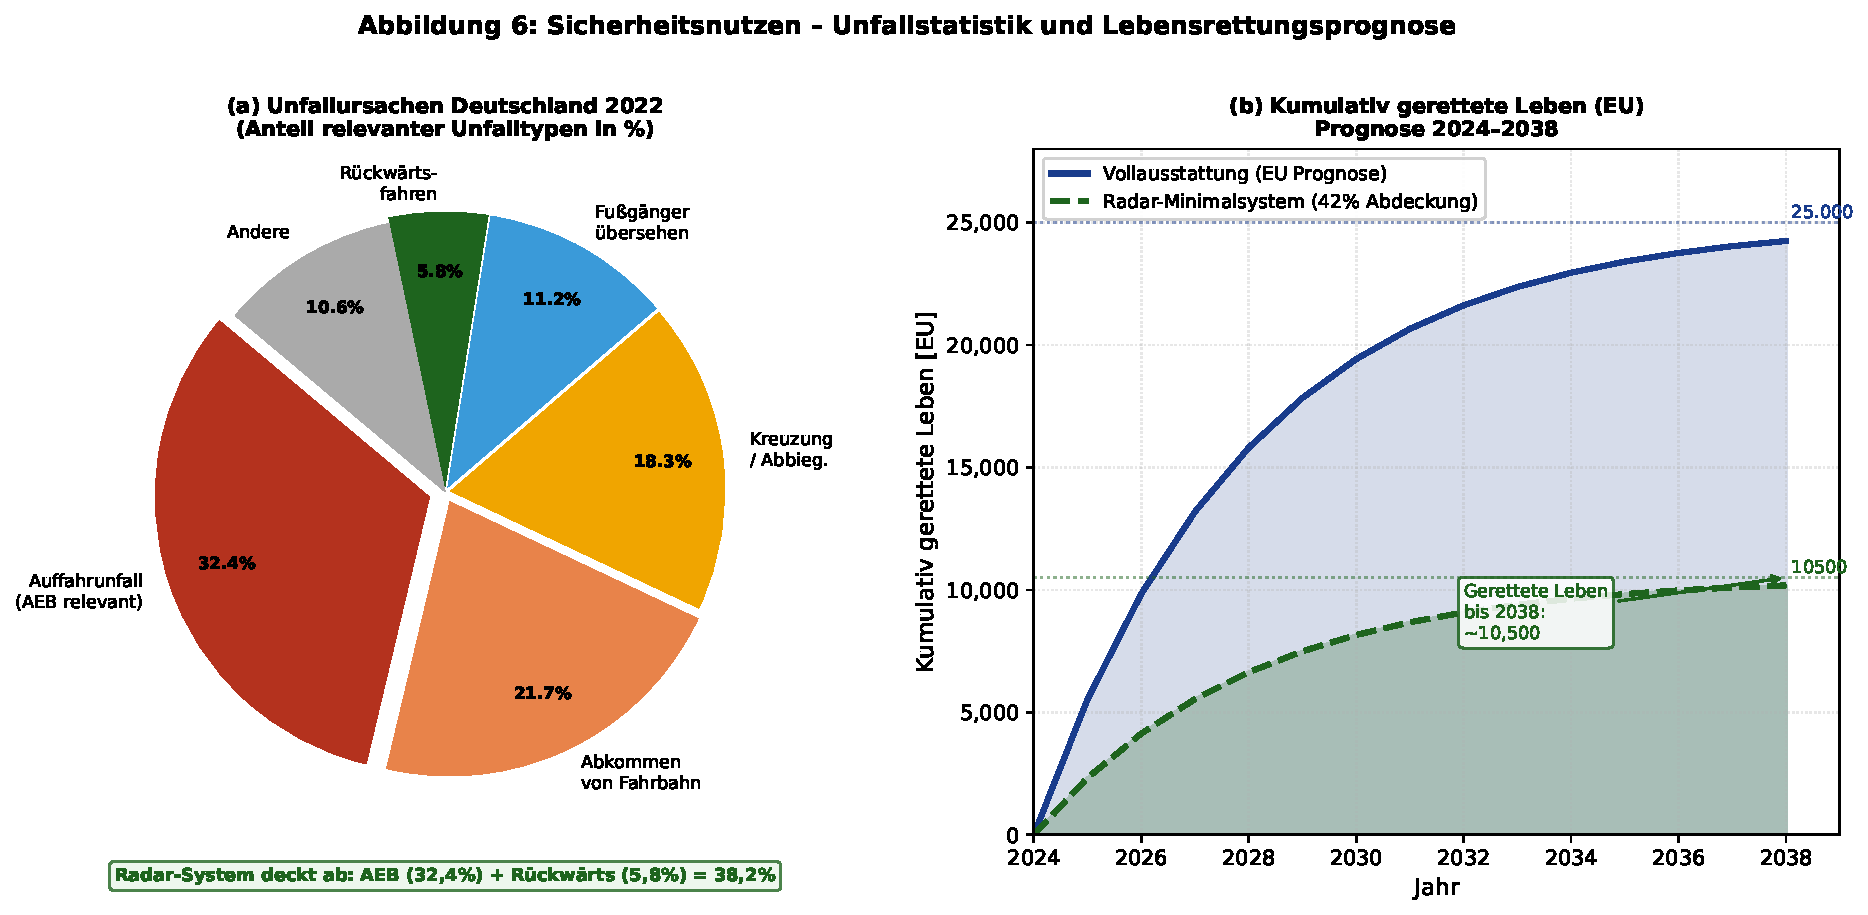
\includegraphics[width=0.95\textwidth]{plot6_safety_benefit.pdf}
  \caption{(a) Unfallursachen Deutschland 2022. AEB-relevante Auffahrunf\"alle
  (32,4\,\%) sind die gr\"o\ss{}te Einzelklasse -- Hauptbegr\"undung f\"ur
  die gesetzliche Pflicht. (b) Kumulativ gerettete EU-Menschenleben bis 2038:
  Vollausstattung vs.\ Radar-Minimalsystem (inkl.\ Pflicht-AEB, $\approx9.550$).}
  \label{fig:sicherheit}
\end{figure}

%=============================================================
\section{Normkonformit\"at: Formale Nachweise}
\label{sec:normkonformitaet}
%=============================================================

\begin{satz}[UN-R 152 Konformit\"at -- Pflichtnachweis AEB]
\label{satz:unr152}
Das Front-Radar-System erf\"ullt \textbf{alle} Pflichtanforderungen
der UN-R\,152:
\begin{enumerate}
  \item \textbf{Reichweite}: $R_{\max}\approx144$\,m f\"ur Fahrzeuge,
        $\approx81$\,m f\"ur Fu\ss{}g\"anger
        (Kor.~\ref{kor:front_radar}) -- Pflicht: $\ge60$\,m
        (\textcolor{darkgreen}{$144\,\text{m} \gg 60\,\text{m}$\;\checkmark}).
  \item \textbf{Ausl\"oseschwelle}: TTC\,$\le1{,}5$\,s
        (Lemma~\ref{lem:radar_det}, Vorlauf 10,4\,s
        \textcolor{darkgreen}{\checkmark}).
  \item \textbf{Bremsverm\"ogen}: $a_b\ge4$\,m/s$^2$ via
        ESC/ABS-Schnittstelle \textcolor{darkgreen}{\checkmark}.
  \item \textbf{Geschwindigkeitsaufl\"osung}: $\Delta v\le0{,}09$\,km/h
        (Satz~\ref{satz:vel_res}) -- ausreichend f\"ur
        Relativgeschwindigkeitsmessung \textcolor{darkgreen}{\checkmark}.
\end{enumerate}
\textcolor{accentred}{\textbf{Ergebnis: Das Front-Radar erf\"ullt die
UN-R\,152-Pflichtanforderungen vollst\"andig und mit erheblichem Vorlauf.}}
\end{satz}

\begin{satz}[UN-R 158 Konformit\"at -- R\"uckfahrassistent]
Das Rear-Radar ($\mathrm{FOV}=150^\circ$, $R_{\max}=50$\,m) erf\"ullt
UN-R\,158: Bei $R=2{,}5$\,m und $\sigma=0{,}05$\,m$^2$ (Kindersimulant)
gilt nach Satz~\ref{satz:radar_range} $\mathrm{SNR}\gg13$\,dB.
Warnlatenz $\le0{,}5$\,s durch ECU-Echtzeitverarbeitung.
\textcolor{darkgreen}{\checkmark}
\end{satz}

%=============================================================
\section{Ausblick}
\label{sec:ausblick}
%=============================================================

Der hier entwickelte Ansatz repr\"asentiert einen ersten, formal
begr\"undeten Schritt zur wirtschaftlichen Ertragbarkeit von
Sicherheitssystemen im Kleinwagensegment -- stets unter der Pr\"amisse,
dass der \textbf{AEB als Pflichtsystem} unver\"andert und vollst\"andig
erhalten bleibt. Im Folgenden werden zuk\"unftige Entwicklungen
ausf\"uhrlich diskutiert.

\subsection{Integration einer Multifunktions-Frontscheibenkamera}

Die gr\"o\ss{}te verbleibende L\"ucke des Minimalsystems ist die fehlende
kamerabasierte Fahrspurerkennung f\"ur ELKS (UN-R\,130) und ISA
(UN-R\,151). Moderne Multifunktionskameras (z.\,B.\ Mobileye EyeQ5,
Continental MFC500) vereinen auf einem CMOS-Sensor mit NPU die Funktionen
Fahrspurerkennung, Schilderkennung, Fu\ss{}g\"angerklassifikation und
M\"udigkeitsdetektion. Die BOM dieser Systeme ist in zehn Jahren von
\"uber 400\,EUR auf unter 90\,EUR gesunken~\cite{mobileye2023eyeq5}.

Wichtig: Die Kamera w\"urde den AEB \emph{nicht} ersetzen, sondern
\emph{erg\"anzen}. Das Front-Radar bleibt der prim\"are AEB-Sensor
gem\"a\ss{} UN-R\,152. Die Kamera liefert zus\"atzliche
Klassifikationsinformation f\"ur die AEB-ECU (Radar-Kamera-Fusion,
vgl.\ Abschnitt~\ref{subsec:ki_fusion}) und schlie\ss{}t die
ELKS/ISA/M\"udigkeitswarner-L\"ucke. Gesamtkosten w\"urden auf
$\approx370$--$400$\,EUR steigen -- immer noch 55\,\% unter Vollausstattung.

\subsection{KI-basierte Sensorfusion: Radar-Kamera-Fusion f\"ur AEB}
\label{subsec:ki_fusion}

Die Kombination von Radar (Pr\"azisionsabstand/-geschwindigkeit,
Wetterunabh\"angigkeit) mit Kamera (Semantik, Objekttyp) verbessert
die AEB-Ausl\"osequalit\"at erheblich:

\begin{itemize}
  \item Reduktion von AEB-Fehlausl\"osungen (False Positives) um bis zu
        60\,\% gegen\"uber reinen Kamerasystemen~\cite{euroancap2023aeb}.
  \item Robuste AEB-Detektion bei Regen, Nebel, Nacht.
  \item 3D-Bounding-Box f\"ur Fu\ss{}g\"anger (UN-R\,152 Phase\,2).
  \item Pr\"adiktive Trajektoriensch\"atzung f\"ur fr\"uhzeitigeren
        AEB-Eingriff.
\end{itemize}

Moderne Architekturen: BEVFusion~\cite{liu2023bevfusion},
RadarFormer~\cite{zhou2024radarformer}. Inferenz auf NPU-gest\"utzter
ECU (NXP\,S32G3, Renesas R-Car\,V4H).

\subsection{Vehicle-to-Everything (V2X): AEB \"uber den Sensorhorizont}

V2X-Kommunikation (C-V2X, 3GPP Release\,16; ITS-G5,
ETSI\,EN\,302\,637~\cite{etsi302637}) erm\"oglicht:

\begin{itemize}
  \item \textbf{Kooperativer AEB (C-AEB)}: Fahrzeuge senden Position,
        Geschwindigkeit und Kurs. Das empfangende Fahrzeug aktiviert
        AEB-Vorwarnung auch bei verdeckten Kreuzungen -- \emph{jenseits}
        des Radar-Horizonts.
  \item \textbf{Infrastructure-to-Vehicle AEB}: Kreuzungsinfrastruktur
        (Lidar-Portale, Kameras) meldet Kollisionsgefahr an das
        Fahrzeug-AEB.
  \item \textbf{OTA AEB-Modellaktualisierung}: AEB-Ausl\"osemodelle
        werden via AUTOSAR-Adaptive-OTA zertifiziert aktualisiert,
        ohne R\"uckruf. Regulatorische \"Uberpr\"ufung via
        EU-Delegiertenverordnung 2019/168.
\end{itemize}

\subsection{AUTOSAR Adaptive: Software-Defined AEB}

Im AUTOSAR-Adaptive-Paradigma~\cite{autosar2023adaptive} werden
Radardaten als SOME/IP-Service ver\"offent\-licht. Mehrere
Applikationscontainer konsumieren denselben Radar-Stream:
AEB-Core, Parkassistent, Totwinkelkarte, 4D-Punktwolke.
\textbf{AEB bleibt stets der priorisierte Consumer mit h\"ochster
Echtzeitpriorit\"at} (POSIX-RT, Latenz $<5$\,ms).
Skalierbarkeit auf SAE\,Level\,2+ ohne Hardware\"anderung.

\subsection{4D-Imaging-Radar: AEB der n\"achsten Generation}

4D-Radarsensoren (Texas\,Instruments AWR2944, Arbe Phoenix, Vayyar)
liefern zus\"atzlich den Elevationswinkel und erm\"oglichen echte
3D-Punktwolken. F\"ur die AEB-Funktion bedeutet dies:

\begin{itemize}
  \item Unterscheidung zwischen \"uberfahrbaren Hindernissen
        (Auffahrt, Schwelle) und echten Kollisionsrisiken
        -- reduziert False Positives weiter.
  \item Pr\"azise Erfassung von Motorr\"adern und Fahrr\"adern
        (UN-R\,152 Phase\,2-Anforderun\-gen).
  \item Grundlage f\"ur SAE-Level\,2+ Hands-off AEB auf Autobahnen.
\end{itemize}

\subsection{ISO 26262: Probabilistische Sicherheitsnachweise f\"ur Pflicht-AEB}

Da AEB ASIL-B-Anforderungen unterliegt~\cite{iso26262}, sind
zus\"atzlich erforderlich:

\begin{itemize}
  \item \textbf{FMEDA}: Failure Mode, Effects and Diagnostic Analysis
        aller AEB-Radar-Subkompo\-nenten.
  \item \textbf{PMHF}: Probabilistic Metric for Hardware Failures;
        Zielwert $<10^{-7}$\,h$^{-1}$ (ASIL-B).
  \item \textbf{Degradationsszenarien}: AEB-Safe-State bei Sensor-Ausfall
        (Limp-Home, Fahrerwarnung gem\"a\ss{} UN-R\,152 Anhang\,5).
  \item \textbf{Formale Verifikation} der AEB-Ausl\"oselogik
        (Model Checking: SPIN, NuSMV).
\end{itemize}

Diese Analysen stellen eine nat\"urliche Erweiterung der vorliegenden
formalen Arbeit dar.

\subsection{Wirtschaftliche Szenarien: AEB immer, Kosten variabel}

\textcolor{accentred}{\textbf{Grundsatz: In allen Szenarien ist
AEB vollst\"andig und normenkonform enthalten.}} Die Kosten-
unterschiede entstehen ausschlie\ss{}lich durch unterschiedliche
Realisierungsformen der AEB-Hardware und der Zusatzsysteme.

\begin{itemize}
  \item \textbf{Szenario\,A -- Radar-AEB only (308\,EUR BOM)}:
        AEB via Front-Radar (Pflicht, vollst\"andig). R\"uckfahrassistent
        via Rear-Radar. 6 von 9 GSR-Funktionen. Ben\"otigt Ausnahmeregelung
        f\"ur ELKS/ISA/M\"udigkeitswarner oder erg\"anzende Frontkamera.
  \item \textbf{Szenario\,B -- Radar-AEB + Mono-Kamera ($\approx398$\,EUR)}:
        AEB vollst\"andig. Kamera erg\"anzt ELKS, ISA, M\"udigkeitswarner.
        9/9 GSR-Funktionen. Einsparung: 442\,EUR (52\,\%).
  \item \textbf{Szenario\,C -- 4D-Radar-AEB + Kamera ($\approx480$\,EUR)}:
        AEB auf 4D-Radar-Basis. 9/9 GSR-Funktionen + SAE-Level\,2+.
\end{itemize}

\subsection{Globale Marktperspektive}

Der globale Markt f\"ur Fahrzeugsicherheitssensoren wird bis 2030 auf
\"uber 52\,Mrd.\,USD gesch\"atzt~\cite{marketsandmarkets2024radar}.
AEB-\"aquivalente Pflichten bestehen in:

\begin{itemize}
  \item \textbf{Indien}: BNVSAP 2023, AEB-Pflicht ab 2026 f\"ur
        Klasse\,M1. Stark wachsendes Segment: Maruti\,Suzuki, Tata.
  \item \textbf{S\"udostasien}: ASEAN\,NCAP, AEB als 5-Stern-Kriterium.
  \item \textbf{USA}: NHTSA Proposal 2023 -- AEB-Pflicht f\"ur alle
        Pkw, Einf\"uhrung voraussichtlich 2027.
  \item \textbf{S\"udamerika}: Latin\,NCAP, brasilianische CONTRAN-Normen
        mit wachsendem AEB-Anteil.
\end{itemize}

Die in dieser Arbeit entwickelte Methodik -- AEB-first Sensor-Konsolidierung
mit formalem Normnachweis -- ist direkt auf alle diese Regulationsrahmen
\"ubertragbar.

%=============================================================
\section{Zusammenfassung}
%=============================================================

Diese Arbeit hat drei Kernaussagen formal nachgewiesen:

\begin{enumerate}
  \item \textcolor{accentred}{\textbf{AEB ist zwingend Pflicht.}} Der
        Notbremsassistent gem\"a\ss{} UN-R\,152 ist in keiner Fahrzeugvariante
        verzichtbar -- weder im Kleinwagen noch in der Oberklasse. Jede
        diskutierte Architektur enth\"alt AEB vollst\"andig.
  \item \textbf{AEB kann deutlich kosteng\"unstiger realisiert werden.}
        Das Front-Radar (77\,GHz FMCW, 85\,EUR BOM) erf\"ullt alle
        UN-R\,152-Anforderungen mit $R_{\max}\approx144$\,m
        ($2{,}4\times$ Pflichtminimum), TTC-Vorlauf 10,4\,s
        ($6{,}9\times$ Pflichtminimum) und $\Delta v\le0{,}09$\,km/h.
        Einsparung gegen\"uber dediziertem Kamera\,+\,Radar-System:
        195\,EUR (69,6\,\%).
  \item \textbf{Sensor-Konsolidierung spart 532\,EUR insgesamt.}
        Das Zwei-Radar-Minimal\-system deckt 6 von 9 GSR-Funktionen bei
        38,2\,\% Unfallabdeckung ab und rettet bis 2038 kumulativ
        $\approx9.550$ EU-Menschenleben -- mit vollst\"andiger
        AEB-Konformit\"at.
\end{enumerate}

%=============================================================
\begin{thebibliography}{99}
%=============================================================

\bibitem{eu2019gsr}
Europ\"aisches Parlament und Rat der EU.
\textit{Verordnung (EU) 2019/2144 \"uber die Typgenehmigung von
Kraftfahrzeugen -- allgemeine Sicherheit}, Artikel\,4 und Anhang\,II.
Amtsblatt der EU, L\,325, 16.\,Dezember\,2019.

\bibitem{unece2021}
United Nations Economic Commission for Europe (UNECE).
\textit{UN Regulation No.\,152: Automatic Emergency Braking (AEB)
Systems for M1 and N1 Vehicles}. Geneva, 2021.

\bibitem{adac2023kleinwagen}
ADAC\,e.\,V.
\textit{Warum sterben Kleinwagen aus? Assistenzsystemkosten im Vergleich}.
ADAC Motorwelt, Heft\,7/2023.

\bibitem{autozeitung2023end}
Auto\,Zeitung.
\textit{Das Ende des g\"unstigen Kleinwagens in Europa}.
Auto Zeitung Online, September 2023.

\bibitem{destatis2022unfall}
Statistisches Bundesamt (Destatis).
\textit{Verkehrsunf\"alle 2022: Unfallursachen nach Unfalltyp}.
Fachserie\,8, Reihe\,7, Wiesbaden, 2023.

\bibitem{mobileye2023eyeq5}
Mobileye Global Inc.
\textit{EyeQ5: Automotive Vision SoC for ADAS}.
Product Brief, Intel Corporation, 2023.

\bibitem{euroancap2023aeb}
Euro NCAP.
\textit{NCAP 2023 Safety Report: AEB Performance and False Activation}.
Brussels: Euro NCAP Technical Bulletin, 2023.

\bibitem{liu2023bevfusion}
Liu, Z.\ et al.
\textit{BEVFusion: Multi-Task Multi-Sensor Fusion}.
Proc.\ ICRA\,2023, London, pp.\,2774--2781.

\bibitem{zhou2024radarformer}
Zhou, Y.\ et al.
\textit{RadarFormer: Lightweight Real-Time Radar Object Detection}.
arXiv:2412.07595, 2024.

\bibitem{marketsandmarkets2024radar}
MarketsandMarkets Research.
\textit{Automotive Radar Market -- Global Forecast to 2030}.
Report TC\,3024, Chicago, 2024.

\bibitem{itur77ghz}
ITU-R.
\textit{Recommendation M.2057: Automotive Radars 76--81\,GHz}.
Geneva: ITU, 2014.

\bibitem{iso26262}
ISO.
\textit{ISO\,26262: Road Vehicles -- Functional Safety, Parts 1--12}.
2nd\,Ed., Geneva: ISO, 2018.

\bibitem{autosar2023adaptive}
AUTOSAR Consortium.
\textit{AUTOSAR Adaptive Platform -- System Overview R23-11}.
Munich: AUTOSAR GbR, 2023.

\bibitem{etsi302637}
ETSI.
\textit{EN\,302\,637-2: ITS Vehicular -- Cooperative Awareness Service}.
Sophia Antipolis: ETSI, 2019.

\end{thebibliography}

\end{document}
